\section{Desenvolvimento}
\subsection{Descrição do sistema}
\begin{frame}{Desenvolvimento}{Descrição do sistema}

Através da técnica classificação de imagem, o presente \textit{software} realiza a extração dos padrões de características de uma imagem. Nessa etapa, o sistema passa por um aprendizado de máquina para extrair os padrões de características que são necessária para atender as necessidades do projeto, que é reconhecer um jogador em campo.

\end{frame}

\begin{frame}{Descrição do sistema}
\begin{figure}
    \centering
    \caption{\label{fig_conversao_img}Etapa de extração de características de uma imagem (A) e seu padrão de características (B).}
    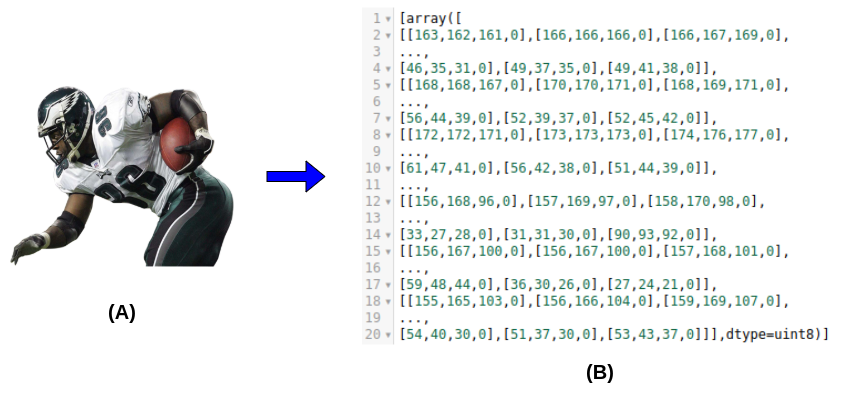
\includegraphics[scale=0.3]{05-SLIDES_DESENVOLVIMENTO/Imagens/conversao-de-imagem.png}
\end{figure}
\end{frame}